\documentclass[a4paper]{article}

\usepackage[utf8]{inputenc}  
\usepackage[francais]{babel}  
\usepackage[top=2cm, bottom=2cm, left=2cm, right=2cm]{geometry}
\usepackage{graphicx}

\begin{document}

\begin{titlepage}
	~ 
	\vfill
	\begin{center}
		\begin{Huge}
			Projet Administration Réseau : \\ Étude d'architecture\\
		\end{Huge}
	\vfill
		\textbf{Hexanôme 4211 :} 
			\\Sandra \bsc{Mondain}, Elisa \bsc{Abidh}, 
			\\Gaël \bsc{Motte}, Armand \bsc{Rossius}, 
			\\Nicolas \bsc{Silva}, Julien \bsc{Levesy}\\
	\vfill
	\end{center}
	\vfill
\end{titlepage}

%\newpage
%\tableofcontents
\newpage

\section{Architecture}

	\subsection{Description} % redétailler en séparant interconnexion et sur chaque site. mettre en avant la sécurité. 	
	
	Afin de mettre en place une communication sécurisée entre les différents sites, nous optons pour une solution basée sur un VPN (Virtual Private Network). 
	
	\paragraph*{} % Routeurs VPN
	L'utilisation du VPN ne concernant que les machines et les automates de l'AIP, nous plaçons sur chaque site de l'AIP un routeur équipé d'un client VPN qui fait la passerelle entre le site et le réseau du campus. Ces routeurs VPN sont également équipés de firewalls. 
	
	\paragraph*{} % Switchs VLAN
	%Comme les automates peuvent être situés dans différentes salles sur chaque site, on mettra en place un sous-réseau par salle, en utilisant des switchs VLAN (Virtual Local Area Network). L'utilisation de ces switchs permet également de limiter le broadcast UDP des automates sur le réseau. 
	Chaque site peut contenir des automates et des PC de travail. On mettra en place un sous-réseau comprenant tous les automates et un autre sous-réseau comprenant tous les PC, en utilisant des switchs VLAN (Virtual Local Area Network). L'utilisation de ces switchs permet de limiter le broadcast UDP des automates sur le réseau. 
	
	\paragraph*{} % DNS 
	Nous allons mettre en place un serveur DNS par site. Ceci permettra de déplacer des plate-formes mobiles d'un site à un autre, car l'utilisation des DNS originaux des campus poserait un problème de réactivité pour la création ou suppression d'une entrée. 
	
	\paragraph*{} % DHCP
	Nous mettrons également en place un serveur DHCP par site pour gérer dynamiquement l'adressage des parcs de machines et d'automates de l'AIP. 
	
	\paragraph*{} % Authentification et Annuaires LDAP
	L'authentification sur site se fera au moyen d'un groupe d'utilisateur répliqué sur tous les annuaires LDAP des différents campus. Ainsi, les utilisateurs mobiles d'un site AIP à l'autre pourront s'authentifier où qu'ils soient. L'authentification depuis l'extérieur pourra se faire grâce à un client VPN déployé sur une machine distante, avec une politique d'authentification par certificat. 
	
	\paragraph*{} % Schéma
	Sur le schéma ci-dessous, on peut voir les différents éléments qui constitueront le réseau. Le tunnel VPN ainsi créé est représenté en rouge. \\
	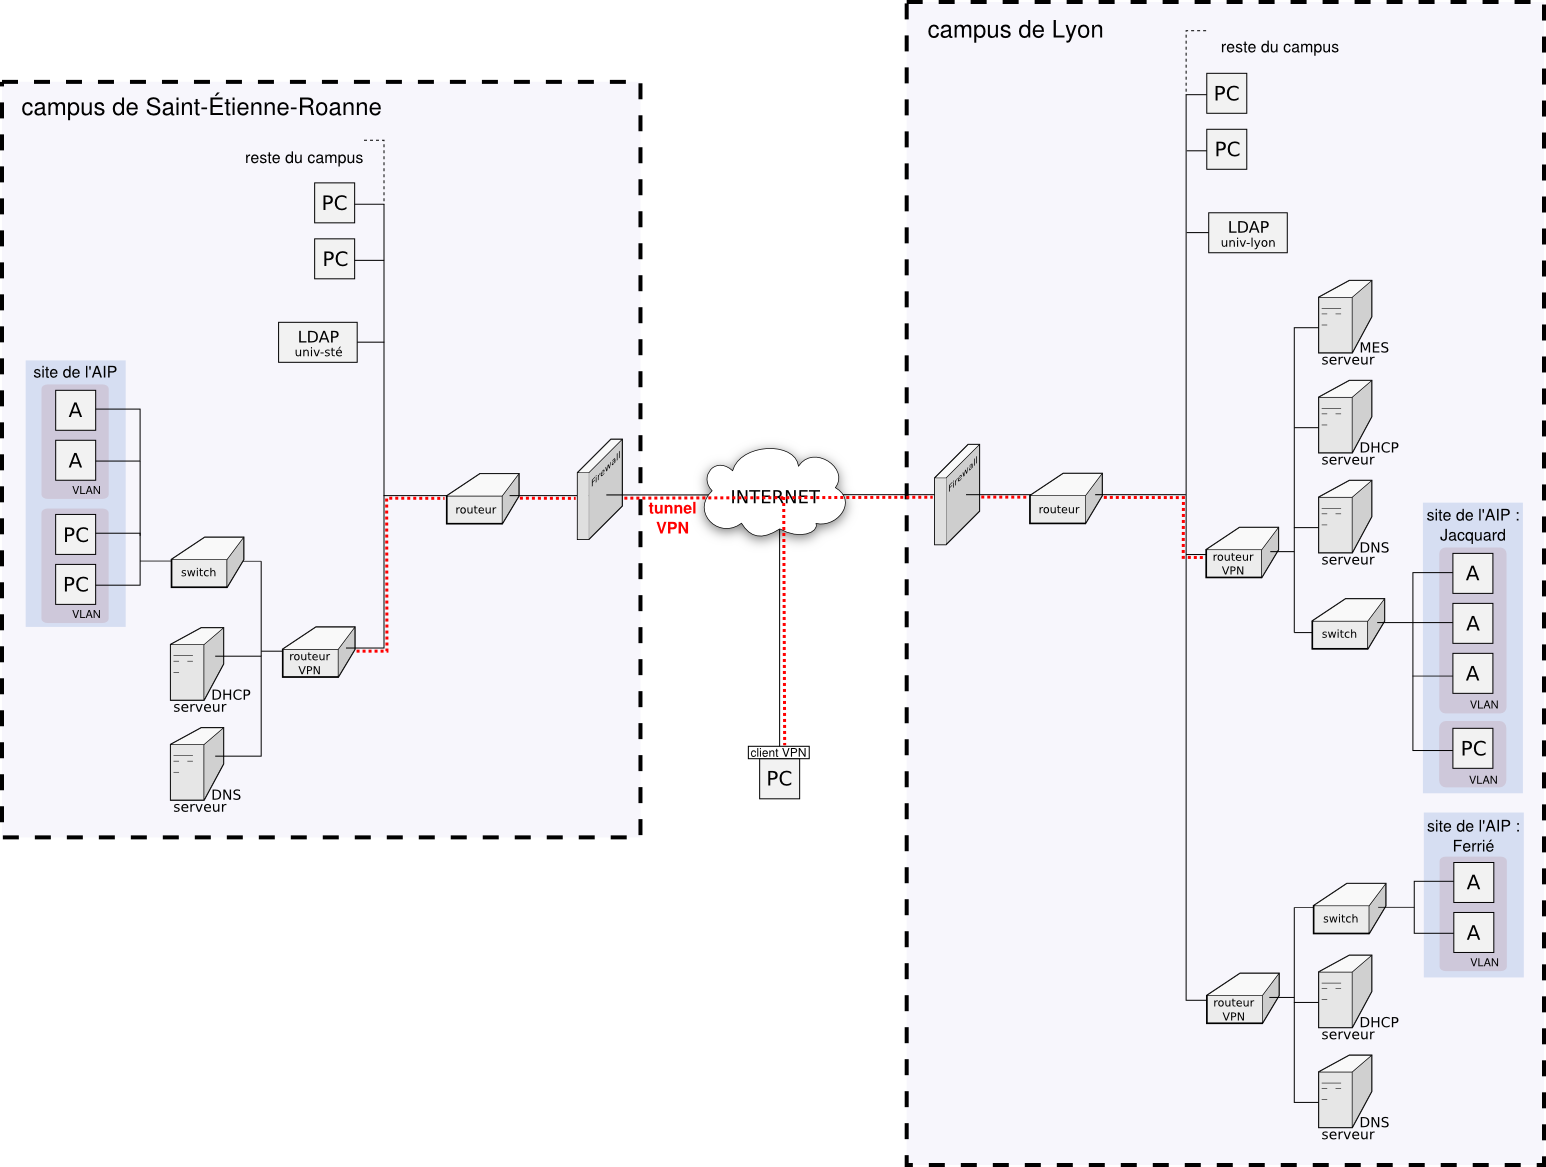
\includegraphics[width=\linewidth]{schema_archi.png}

	
\section{Plans de nommage et d'adressage}
	\subsection{Plan de nommage}

	Pour rappel, les exigences au niveau du plan de nommage sont :\\
	\begin{itemize}
	\item Gestion des campus
	\item Gestion des sites présents dans les campus
	\item Type l'entrée
	\item Générique et extensible
	\end{itemize}	

	Afin de répondre aux différentes exigences de nommage des machines nous proposons le plan de nommage suivant.	
	
	\textbf{Campus-Site-Type-Nom}	
	
	\begin{description}
	\item[Campus]\hfill\\
	Il s'agit ici d'un acronyme sur 4 caractères désignant les campus (sites géographiques) possédant les ateliers AIP.\\
	
	\item[Site]\hfill\\
	Nom de site commençant par les lettres "AIP", puis le nom du batiment, puis le numéro de l'atelier si il existe plusieurs ateliers par batiments.
	
	\item[Type]\hfill\\
	Type de la machine reliée au réseau\\
	Si c'est un serveur, le service hébergé par ce dernier\\
	Si c'est une salle, on indique le numéro de salle préfixé du caractère 'S'\\
	
	\item[Nom]\hfill\\
	Nom de la machine par type, numéro unique.
	\end{description}	
	
	\textit{Exemples : INSA-AIPJacquard-A-02, ROAN-AIPMachin2-S03-04, INSA-AIPFerrie-S03-02}	
	
	\subsection{Plan d'adressage}
	
	% TODO insérer le formidable diagrame par site
	
	
\end{document}
